%!TEX root = ../dissertation.tex
\chapter{Problem Description} \label{cha:problem_description}

The problem addressed in this project takes inspitaion from the classical blocks world problem\footnotemark{}. 
\footnotetext{\url{https://en.wikipedia.org/wiki/Blocks_world\#:~:text=In\%20its\%20basic\%20form\%2C\%20the,different\%20sizes\%2C\%20shapes\%20and\%20colors.}}
The blocks world is a planning domain in artificial intelligence and is used as a toy problem. From an algorithm perspective, it is an NP-Hard search and planning problem \cite{Gupta1991ComplexityRF, Chenoweth1991OnTN}.
Here, a more general version of it is presented. \\
First of all, the environment consists of:
\begin{itemize}
	\item A robot manipulator, equipped with a video camera;
	\item Blocks (cubes) of the same size, which all have an AprilTag \cite{olson2011tags, wang2016iros} marker attached to one of their faces;
	\item Zero or more fixed objects, also equipped with the AprilTag markers.
\end{itemize}

\begin{figure} [h]
\centering
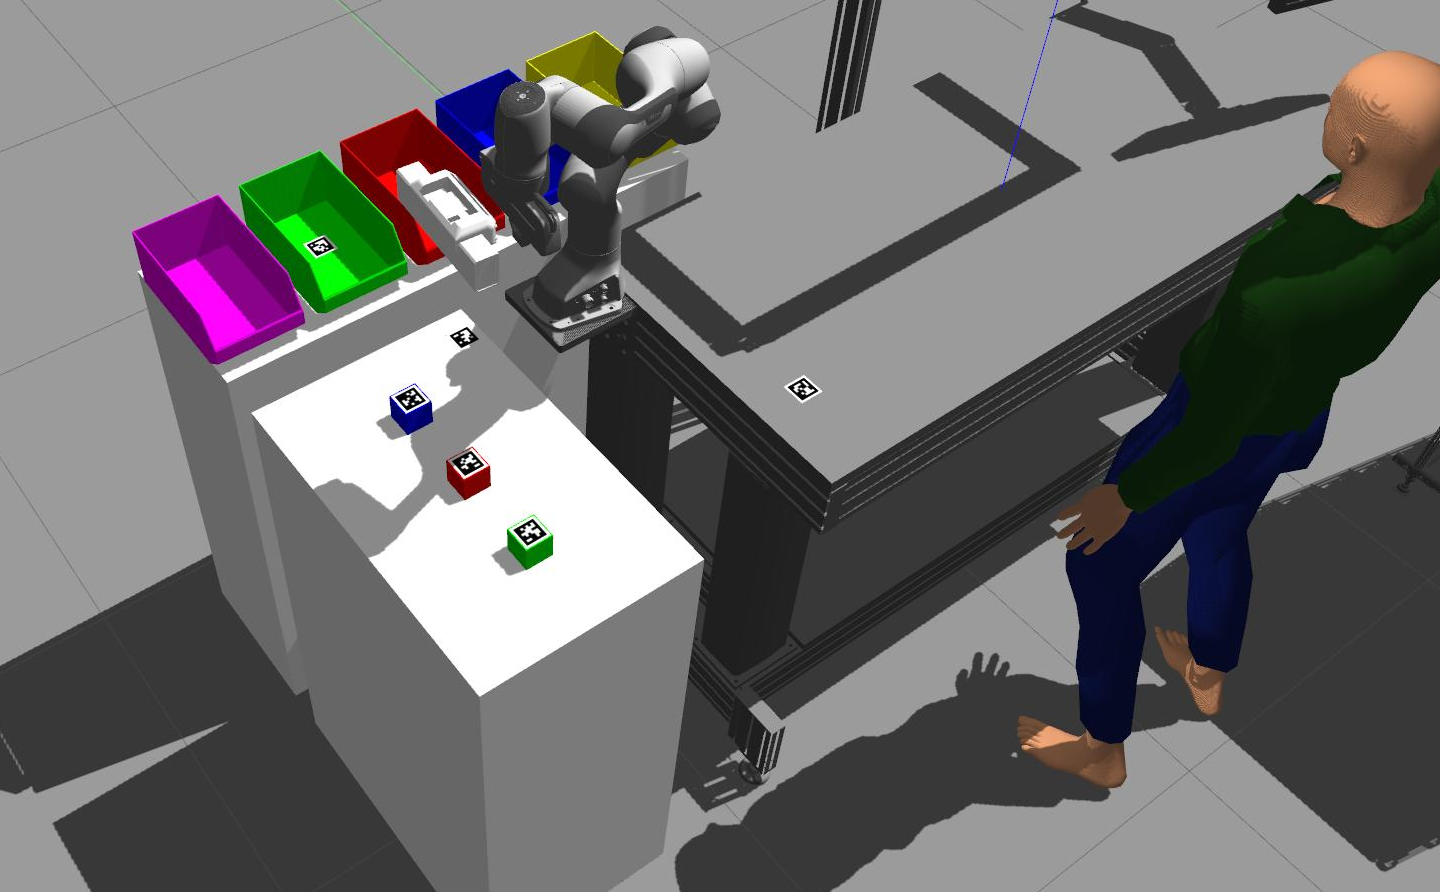
\includegraphics[width=1.0
\textwidth]{figures/Magistrale/env_fin_1}
\caption[Environment Configuration]{The configuration of the environment used in this project: a white table on the left, a grey workbench on the right, on which the robot manipulator is fixed, and behind it, five bins of various colours, which will contain the different blocks. All these objects have an AprilTag on top of each one.
\label{fig:env_1}}
\end{figure} 

Figure \ref{fig:env_1} illustrates a possible configuration of the environment, which is the one used in this project. \\
Compared to the state-of-the-art, where the robot arm has to pick and place the blocks and the goal is to build one or more vertical stacks of them, the goal is generalized in a way that any arrangement of the blocks can be achieved. 
That is, given any initial arrangement of the blocks in the environment, the goal is finding the shortest sequence of actions that the robot has to perform to achieve the target arrangement. \\
To define the implementation, it is first necessary to explain the constraints of this problem:

\begin{itemize}
	\item The robot knows only four actions: \textit{Pickup}, \textit{Putdown}, \textit{Stack}, \textit{Unstack};
	\item Each block is \textit{clear} if and only if it has no object on it and is not \textit{in-hand} (i.e., the robot's hand can take it with a single action);
	\item Each block can be \textit{on} the table, on the top of another object or \textit{in-hand};
	\item The robot's hand may be busy (it is holding a block) or free (it holds nothing);
	\item Only one block can be picked up at a time, putting it down before the next. It is not possible to pick up a block that is under another one (because it is not considered \textit{clear}) or to move a fixed object.
\end{itemize}

The \textit{Pickup} action is the opposite of \textit{Putdown} and they are used to take/place a block from/on a fixed object. The \textit{Stack} action is the opposite of \textit{Unstack} and they are used to put/take a block on/from another block or a fixed object. \\
Figure \ref{fig:blocks_example} illustrates an example. Consider two blocks (A and B) on a table and block A is \textit{on} block B: to pick up block B, that block must be \textit{clear} and the hand must be free. Initially, block A is \textit{clear}, while B is not (Subfigure 1 of Figure \ref{fig:blocks_example}). Thus, one can do \textit{Unstack} of blocks A and B, getting block B \textit{clear} and block A \textit{in-hand} (Subfigure 2 of Figure \ref{fig:blocks_example}), then do \textit{Putdown} of block A (Subfigure 3 of Figure \ref{fig:blocks_example}) and finally do \textit{Pickup} of block B, achieving the goal (Subfigure 4 of Figure \ref{fig:blocks_example}).

\begin{figure} [h]
\centering
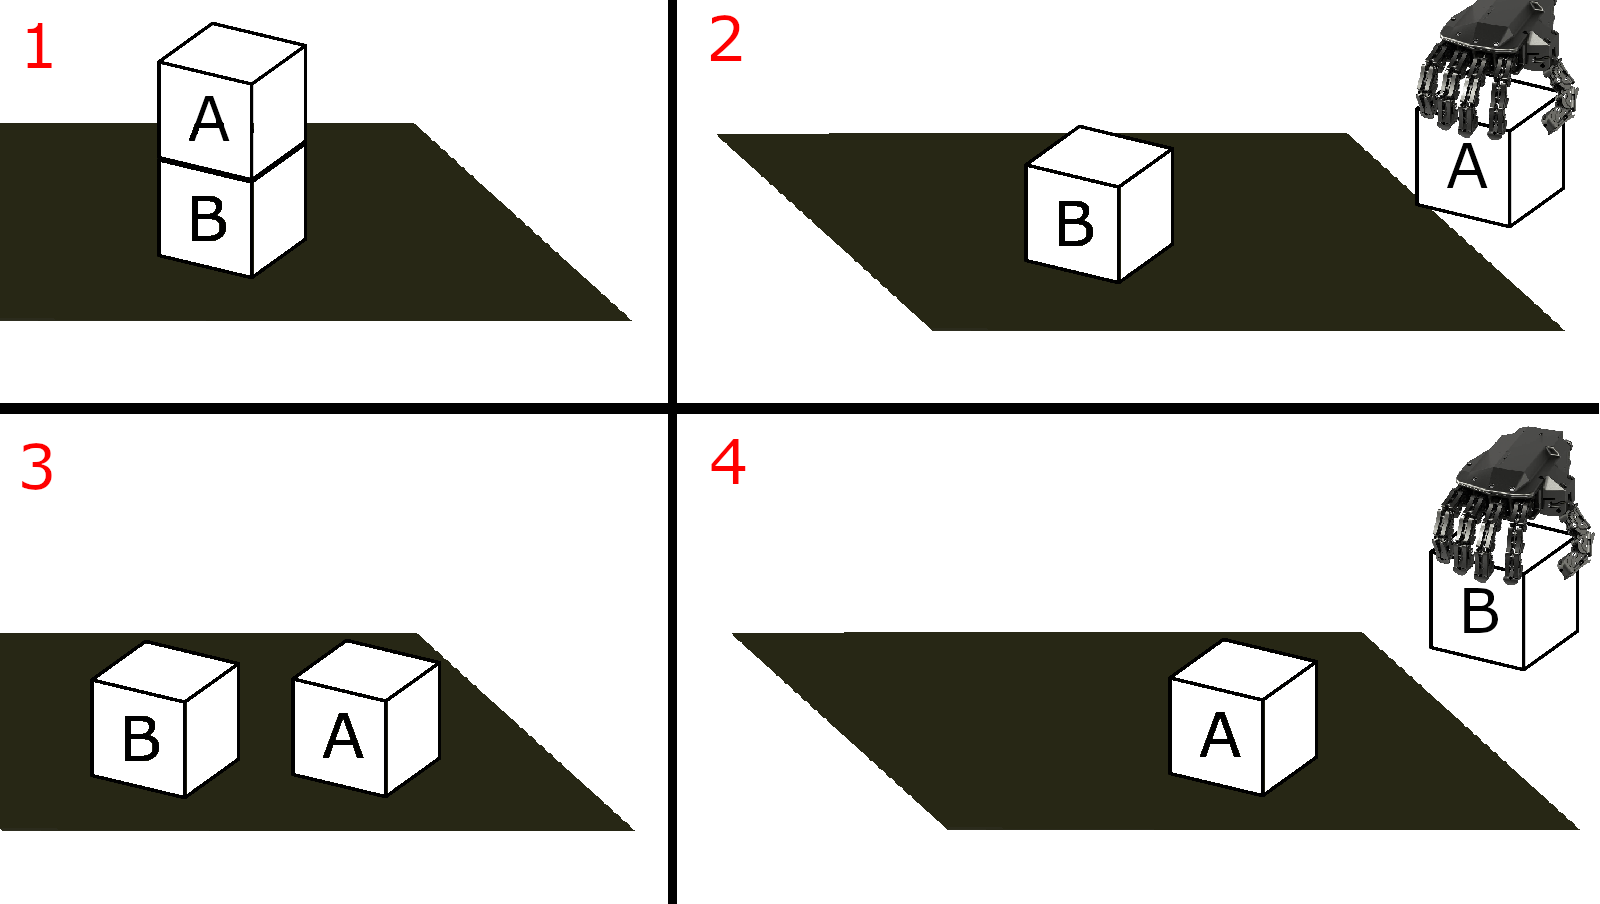
\includegraphics[width=0.9
\textwidth]{figures/Magistrale/blocks_example}
\caption[Blocks world example]{Three actions to go from state 1 (initial arrangement) to state 4 (target arrangement): \textit{Unstack} of A and B, \textit{Putdown} of A, \textit{Pickup} of B. 
\label{fig:blocks_example}}
\end{figure} 

Since it is possible to have more fixed objects (such as tables, workbench, etc.) than in the blocks world, where there is only a work plane, any free block can always be considered on top of something else. Consequently, the actions \textit{Pickup} and \textit{Putdown} lose their meaning because they become subcases of the respective \textit{Unstack} and \textit{Stack}. However, in this project all four are still maintained and used, as explained below. 


\section{Knowledge Base in Atomese}\label{sec:env_atomese}

Any aspect of the environment, the problem, the robot or anything else can be represented in the form of atoms, which will populate the AtomSpace (i.e., the hypergraph of the KB). \\
There are many different ways of encoding these aspects. The one used in this project is proposed below. \\

Firstly, the Atomese representation of the objects is \\
\begin{python}
	(InheritanceLink
		(ConceptNode "screw")
		(ConceptNode "object"))

	(InheritanceLink
		(ConceptNode "table")
		(ConceptNode "fixed-object"))
\end{python}
On a practical (physical) level, the objects will all be cubes, except for the fixed ones. At the conceptual level, a semantic meaning will be associated to the AprilTag marker of each cube. In this way, and thanks to the AprilTags, it is possible to simplify the perception and manipulation of objects by replacing each different object with a cube. \\
In other words, it will be possible to \enquote{simulate} working with any kind of object, and thus demonstrate the potential of the NLP aspect of this project, leaving out perception and manipulation, which do not concern it at the moment. \\
For this reason, the code above speaks of \textit{screw} and not \textit{cube\_1}. \\

In that code, the \textit{screw} has been defined as an \textit{object} and the \textit{table} as a \textit{fixed-object}. 
ConceptNodes were used to refer to \enquote{concepts} and InheritanceLinks to connect two ConceptNodes with an \enquote{inheritance} meaning. This way, when the robot searches for which objects it can move, it will limit the pattern matching only to atoms that are objects (thus, only to the screw). \\
As each atom is unique, it is not necessary to first define objects (i.e., \textit{screw} and \textit{table}) and concepts (i.e., \textit{object} and \textit{fixed-object}) and then, link them. Within the same AtomSpace, once an atom is defined, whether independently or within any hypergraph, it will remain unique and the creation of other hypergraphs containing that atom will not create a new one, but rather it will be shared between the various hypergraphs, in a sense, connecting them. \\

In addition, by construction of pattern matching rules, it is necessary to explicitly define the \enquote{non-equality} between all the various pairs of objects. Therefore, for example, given three objects such as \textit{screw}, \textit{bolt} and \textit{table}, there will be atoms like these: \\
\begin{python}
	(NotLink (EqualLink 
		(ConceptNode "screw") (ConceptNode "bolt")))

	(NotLink (EqualLink 
		(ConceptNode "screw") (ConceptNode "table")))

	(NotLink (EqualLink 
		(ConceptNode "bolt") (ConceptNode "table")))
\end{python}
They correspond to all possible simple combinations (without repetition) that can be constructed from the set of all objects (fixed ones included) taken two at a time. \\

Finally, now that the objects have been constructed, inherited and differentiated, one or more states must be associated with them. The best way to represent the state of an object is via an EvaluationLink, which associates a PredicateNode with one or more objects (their relative atoms). The possible states of an object are: \textit{clear}, \textit{in-hand}, \textit{on}. Thus, for example: \\
\begin{python}
	(EvaluationLink
		(PredicateNode "clear")
		(ConceptNode "bolt"))
	
	(EvaluationLink
		(PredicateNode "in-hand")
		(ConceptNode "screw"))
	
	(EvaluationLink
		(PredicateNode "on")
		(ListLink
			(ConceptNode "bolt")
			(ConceptNode "table")))
\end{python}

In Appendix A, Section \ref{sec:KB_examples}, a complete examples have been added for further details.
%%  ovviamente si possono aggiungere un sacco di stati, attributi, etc. in più

\section{Actions in Atomese}\label{sec:domain_atomese}
Once the atoms relative to the objects have been defined, the robot's actions must also be defined as hypergraphs. 
From this point on in the paper, these actions will also be called \enquote{rules}, being called rules the ones that are executed within AtomSpace for pattern matching. \\
Before exposing them, Section \ref{sec:PDDL} in Appendix A provides the domain and problem in Planning Domain Definition Language (PDDL) notation of the standard block world problem.
Automated planning and scheduling problems are usually described in the PDDL notation, which is an AI planning language for symbolic manipulation tasks.
Starting from those definitions of the various actions, one can better understand how they are created in Atomese. \\

Each action used in this project, as in the PDDL notation, requires preconditions and applies effects, which are described as follow:

\begin{itemize}

	\item \textbf{Pickup} a block from the initial fixed object. \\
Preconditions:
	\begin{itemize}
		\item block must be clear
		\item block must be an object
		\item block must not be \enquote{stacked}
	\end{itemize}
Effects:
	\begin{itemize}
		\item block no longer clear
		\item block is in hand
	\end{itemize}

	\item \textbf{Putdown} a block from the hand to a fixed object. \\
Preconditions:
	\begin{itemize}
		\item block must be in hand
		\item block must be an object
	\end{itemize}
Effects:
	\begin{itemize}
		\item block is clear
		\item block no longer in hand
	\end{itemize}

	\item \textbf{Stack} block A on top of the block B. \\
Preconditions:
	\begin{itemize}
		\item block A must be different from block B
		\item block A must be an object
		\item block A must be in hand
		\item block B must be a clear object or must be a fixed object
	\end{itemize}
Effects:
	\begin{itemize}
		\item block A is on top of block B
		\item block A is \enquote{stacked}
		\item block A no longer in hand
		\item block A is clear
		\item block B no longer clear (if it is an object)
	\end{itemize}

	\item \textbf{Unstack} block A from the top of block B. \\
Preconditions:
	\begin{itemize}
		\item block A must be different from block B
		\item block A must be an object
		\item block A must be clear
		\item block A must be on top of block B
		\item block B must be an object or a fixed object
	\end{itemize}
Effects:
	\begin{itemize}
		\item block A is in hand
		\item block A no longer clear
		\item block A no longer on top of block B
		\item block A no longer \enquote{stacked}
		\item block B is clear
	\end{itemize}
\end{itemize}
%% TODO appendice A scrivi qualcosa sulle regole + regola extra
Only the \textit{Pickup} rule is presented and explained here, as an example, whereas the code of the other three can be found in Appendix A, Section \ref{sec:action_atomese}. \bigskip \\
\begin{footnotesize}
\textbf{Code in Atomese notation:} \\
\textit{Pickup} action rule.
\end{footnotesize}

\begin{python}
(define (pickup-action . args)
  (define precond (car (cdr args)))
  (define eff (car args))
  (cog-extract-recursive! precond)
  eff
)

(define (pickup args)
  (let 
    ((rule
      (if (equal? args `())
        (QueryLink
          (VariableList
            (TypedVariableLink 
              (VariableNode "?ob") 
              (TypeNode "ConceptNode"))
          ) ; parameters
          (AndLink
            (PresentLink
              (InheritanceLink
                (VariableNode "?ob")
                (ConceptNode "object"))
              (EvaluationLink
                (PredicateNode "clear")
                (VariableNode "?ob"))
            )
            (AbsentLink
              (EvaluationLink
                (PredicateNode "stacked")
                (VariableNode "?ob"))
            )
          )
          (ExecutionOutputLink
            (GroundedSchemaNode "scm: pickup-action")
            (ListLink
              ; effect
              (EvaluationLink
                (PredicateNode "in_hand")
                (VariableNode "?ob"))
              ; precondition
              (EvaluationLink
                (PredicateNode "clear")
                (VariableNode "?ob"))
            )
          )
        )
        (QueryLink
          (VariableList
            (TypedVariableLink 
              (VariableNode "?ob") 
              (TypeNode "ConceptNode"))
          ) ; parameters
          (AndLink
            (PresentLink
              (InheritanceLink
                (VariableNode "?ob")
                (ConceptNode "object"))
              (EvaluationLink
                (PredicateNode "clear")
                (VariableNode "?ob"))
            )
            (EqualLink
              (VariableNode "?ob")
              args
            )
            (AbsentLink
              (EvaluationLink
                (PredicateNode "stacked")
                (VariableNode "?ob"))
            )
          )
          (ExecutionOutputLink
            (GroundedSchemaNode "scm: pickup-action")
            (ListLink
              ; effect
              (EvaluationLink
                (PredicateNode "in_hand")
                (VariableNode "?ob"))
              ; precondition
              (EvaluationLink
                (PredicateNode "clear")
                (VariableNode "?ob"))
            )
          )
        )
      )
    ))
    rule
  )
)
\end{python}

The code is divided into two functions: \textit{(pickup-action . args)} and \textit{(pickup args)}. \\
The main rule (or action or function) is the second one, called \textit{pickup} (line 8), which describes the action of picking up some object.
It is composed of two large QueryLink atoms (lines 12 and 47), as for all other actions. \\
Only one of the two atoms is used for each call to this function, through the `if' conditional construct (line 11). It checks whether the function has an argument \textit{args} other than empty \textit{'()}. 
If it is indeed empty, then the QueryLink from line 12 to 46 is used, otherwise the one from line 47 to 85, which actually uses the \textit{args} argument.
Indeed, the variable \textit{rule} is defined as one of the two QueryLinks, depending on the result of the conditional construct, and then, it is applied in line 88. \\
These QueryLinks are completely identical, except for the EqualLink atom on line 62.
Consequently, take a look first at the QueryLink without arguments, based on the generic description of a QueryLink in Section \ref{sec:atoms}. \\

Its variable\_declaration part consists of a \textit{?ob} parameter (VariableNode) that is restricted to the ConceptNode type (lines 13-17). 
In this way, the rule will do pattern matching using the conditional part as a pattern, which will be parameterized by \textit{?ob} that will result as all possible objects that can be picked up, given the current composition of the AtomSpace. Thus, the notation "object (parameterized)" is given to generic objects that satisfy the parameterization requirements. \\

The conditional part (or pattern) requires that the logical AND (AndLink) be evaluated to TRUE (lines 18-32). This can only happen when both PresentLink and AbsentLink are evaluated to TRUE at the same time. 

\begin{itemize}
	\item AbsentLink is a trick to differentiate atoms simply \textit{clear} from those \textit{clear}, but also \textit{on} some other object; this corresponds to differentiating \textit{Pickup} and \textit{Unstack} actions (design choice). \\
Briefly, when an object is subjected to a \textit{Stack} action, a \enquote{stacked} state atom is created, and when it is subjected to \textit{Unstack}, that atom is removed from AtomSpace. \\
Finally, AbsentLink checks for the absence of that atom in AtomSpace: if the object (parameterized) is simply \textit{clear}, then the atom is not there and it can be picked up, otherwise the object (parameterized) is \textit{on} something else and the \textit{Unstack} action must be used instead of \textit{Pickup}. 
	\item PresentLink, the opposite of AbsentLink, checks for the presence of atoms composing it in the AtomSpace , just like logical AND, returns TRUE only when all are found. \\
In this case, it verifies that the object (parameterized) is indeed an \textit{object} and that it is also \textit{clear}, from the definitions of the Pickup action.
\end{itemize}

The last part of the QueryLink (lines 33-45) is relative to the graph re-write and uses an ExecutionOutputLink atom to execute a GroundedSchemaNode. The GroundedSchemaNode type atom behaves like the GroundedPredicateNode described in the previous section, but it is not associated with an EvaluationLink, it simply executes a Schema or Python code or Combo procedure. The preference of GroundedSchemaNode, over GroundedPredicateNode, is a design choice to follow the PDDL definition of the various actions. \\
In this project, it was decided to use a Schema code (line 34, `scm' stands for Schema) that executes the \textit{pickup-action} function, with a list of arguments provided by the ExecutionOutputLink. \\
This list of arguments (line 35) is made up of the effect and precondition of the Pickup rule. Thus, the rule wants the object (parameterized) to be \textit{clear}, as a precondition, and the effect corresponds to the atom describing the \textit{in-hand} state of the object . 
Initially, a QueryLink structure was sought that would also work using inference, specifically backward chaining. Thus, only one atom each was accepted for preconditions and effects. Although ExecutionOutputLink uses a ListLink, which can contain multiple arguments, this design was retained considering a possible integration of an inference algorithm to solve the problem. Consequently, the remaining effects and preconditions not included in the ListLink are added and removed in the called function. \\
The \textit{pickup-action} called function (lines 1-6) takes these two atoms as arguments, removes the one corresponding to the precondition from the AtomSpace and finally applies the effect, creating the corresponding atom in the AtomSpace (some other functions add more effects and remove more preconditions). This is how the action takes place inside the AtomSpace: states that would no longer be \enquote{valid}, after the action has been performed ,are removed (such as the state of \textit{clear}, because the object (parameterized) will be in hand, thus no longer \textit{clear}) and those created due to the action are added (such as the state of \textit{in-hand}). \\

Now that the first QueryLink has been explained, the second behaves in the same way, but with an additional constraint in the conditional part. \\
This constraint is the EqualLink in line 62 and it is used to limit the parameter (the VariabileNode) to coincide with the \textit{args} argument, which will be an atom corresponding to the object to be picked up, effectively restricting the pattern matching to that single atom. \\
In practice, the QueryLink without argument performs the Pickup action on all objects that can actually be picked up, instead of the QueryLink with argument that does \textit{Pickup} only of the object passed as argument. That is, the first shows which objects are pickable, the second actually picks one of them. \\
The reason why these two possibilities (QueryLinks) are necessary will be better understood when the algorithm is discussed (Section \ref{sec:step_search}). 

 